\section{Overview}
\label{sec:overview}

In this section we present an overview of the methodology for
computing heap summaries lazily for generalized symbolic execution
and illustrate its application to a small example. We begin with
a brief explanation of the two supporting technologies.

\subsection{Generalized Symbolic Execution}

The traditional notion of symbolic 
execution~\cite{clarke76TSE,King:76} was developed in the
context of sequential programs with a fixed number of program
variables having primitive types, e.g., integer, Boolean.
\emph{Generalized Symbolic Execution (GSE)}~\cite{GSE03} extends
traditional symbolic execution to enable analysis of heap
manipulating software written in commonly used imperative
languages such as Java and C++. 
GSE enables context and flow sensitive analysis of complex
and potentially unbounded data structures by
constructing the heap ``lazily'' during symbolic execution,
generating potential heap structures based on program semantics.
The original GSE algorithm uses lazy initialization in which
symbolic execution explores different heap structures
by materializing the heap at the first memory access (read) of
an uninitialized symbolic object. At this point, a non-deterministic
choice point of heap locations is created that includes three cases:
(1) a null
object, (2) a new instance of the object, and (3) aliases
to other type-compatible symbolic objects that have been materialized
along the same execution path~\cite{GSE03}.  
Improvements to the original lazy initializtion algorithm include the 
\emph{lazier} and \emph{lazier\#} algorithms~\cite{Kiasan06,Kiasan07}
%implemented as part of the \emph{Bogor$/$Kiasan} framework, 
which
reduce the amount of nondeterminism in the lazy algorithm by
delaying initialization, sometimes indefinitely. 
Although the lazy initialization algorithms extend symbolic
analysis to heap manipulating software through partially initialized
structures created on-the-fly, the materialization process
exacerbates the state space explosion problem in symbolic
execution and may generate
heap structures which, because of their size, exceed the capabilities
of the materialization technique.

\subsection{Heap Summarization Techniques}

\subsection{Our Approach}

Consider the code for a (partial) {\tt LinkedList} implementation
shown in~\figref{fig:example}. 
Generalized Symbolic Execution will materialize the heap by adding
non-deterministic choice points representing the different potential heap
configurations at each location in the program where a field is read.
The number of choice points introduced by each field access is dependent
on how many type compatible heap locations were materialized during 
previous field reads on the current path
and on the lazy initialization algorithm used by GSE. 
The graph shown in~\figref{fig:tvc} illustrates the growth in the symbolic
execution state space 
in terms of time as the number of calls to the {\tt contains()} method which
reads the {\tt head} field.
The blue and green lines show growth for the lazy and lazier\# 
initialization algorithms respectively.
Notice that the runtime, i.e., non-determinism, increases rapidly with 
only a small number of invocations of the {\tt contains()} method
with the lazy and lazier\# approaches.

Our technique, blah, builds on the lazy initialization algorithm for
Generalized Symbolic Execution by materializing the heap on-the-fly, i.e.,
``lazily'' during symbolic execution, but
and heap summariesOur approach is inspired by two state-of-the-art techniques: Generalized 
Symbolic Execution (GSE) and heap summarization techniques. Like GSE,
our approach constructs the heap lazily, i.e., materializing the heap
on-the-fly during symbolic execution. However, unlike GSE, we create
a compact representation of the heap, i.e., a heap summary, which eliminates
isomorphic heap shapes without losing precision. The heap summaries computed
by our approach have two important advantages: 1) they are capable of 
handling arbitrary data structures, including recursive data structures,
and, 2) because of lazy initialization, dynamic bounding can be use to
bound input data structures.

\begin{figure}
\begin{tabular}[c]{l}
\begin{lstlisting}
public class LinkedList {

/** assume the linked list is valid with no cycles **/
LLNode head;
Data data0, data1, data2, data3, data4;

private class Data { Integer val; }

private class LLNode {
  protected Data elem;
  protected LLNode next; }

public static boolean contains(LLNode root, Data val) {
  LLNode node = root;
  while (true) {
    if(node.val == val)  return true;
    if(node.next == null) return false;
    node = node.next;
}}

public void run() {
if(LinkedList.contains(head, data0) && LinkedList.contains(head,data1) &&
   LinkedList.contains(head, data2) && LinkedList.contains(head, data3) &&
   LinkedList.contains(head, data4)) return;}}
\end{lstlisting}
\end{tabular} 
\caption{Linked list}
\label{fig:example}
\end{figure}

\begin{figure}[htb]
\scalebox{0.45}
{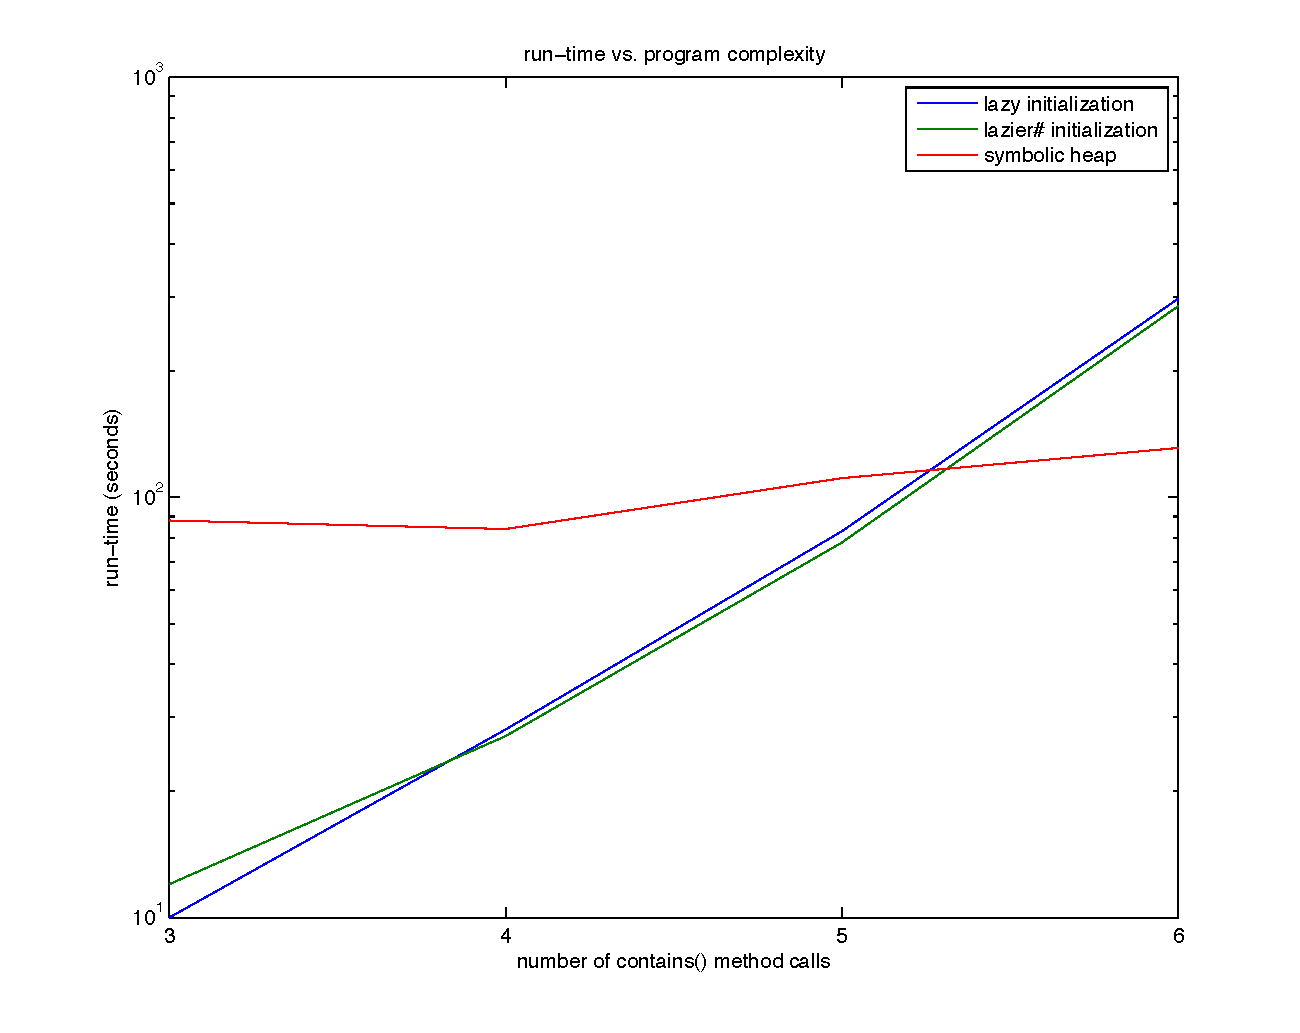
\includegraphics[width=563px]{../figs/time_vs_complexity.pdf}}
\caption{Time versus complexity for the linked list example}
\label{fig:tvc}
\end{figure}

